\chapter{Дешифратор}

\begin{center}
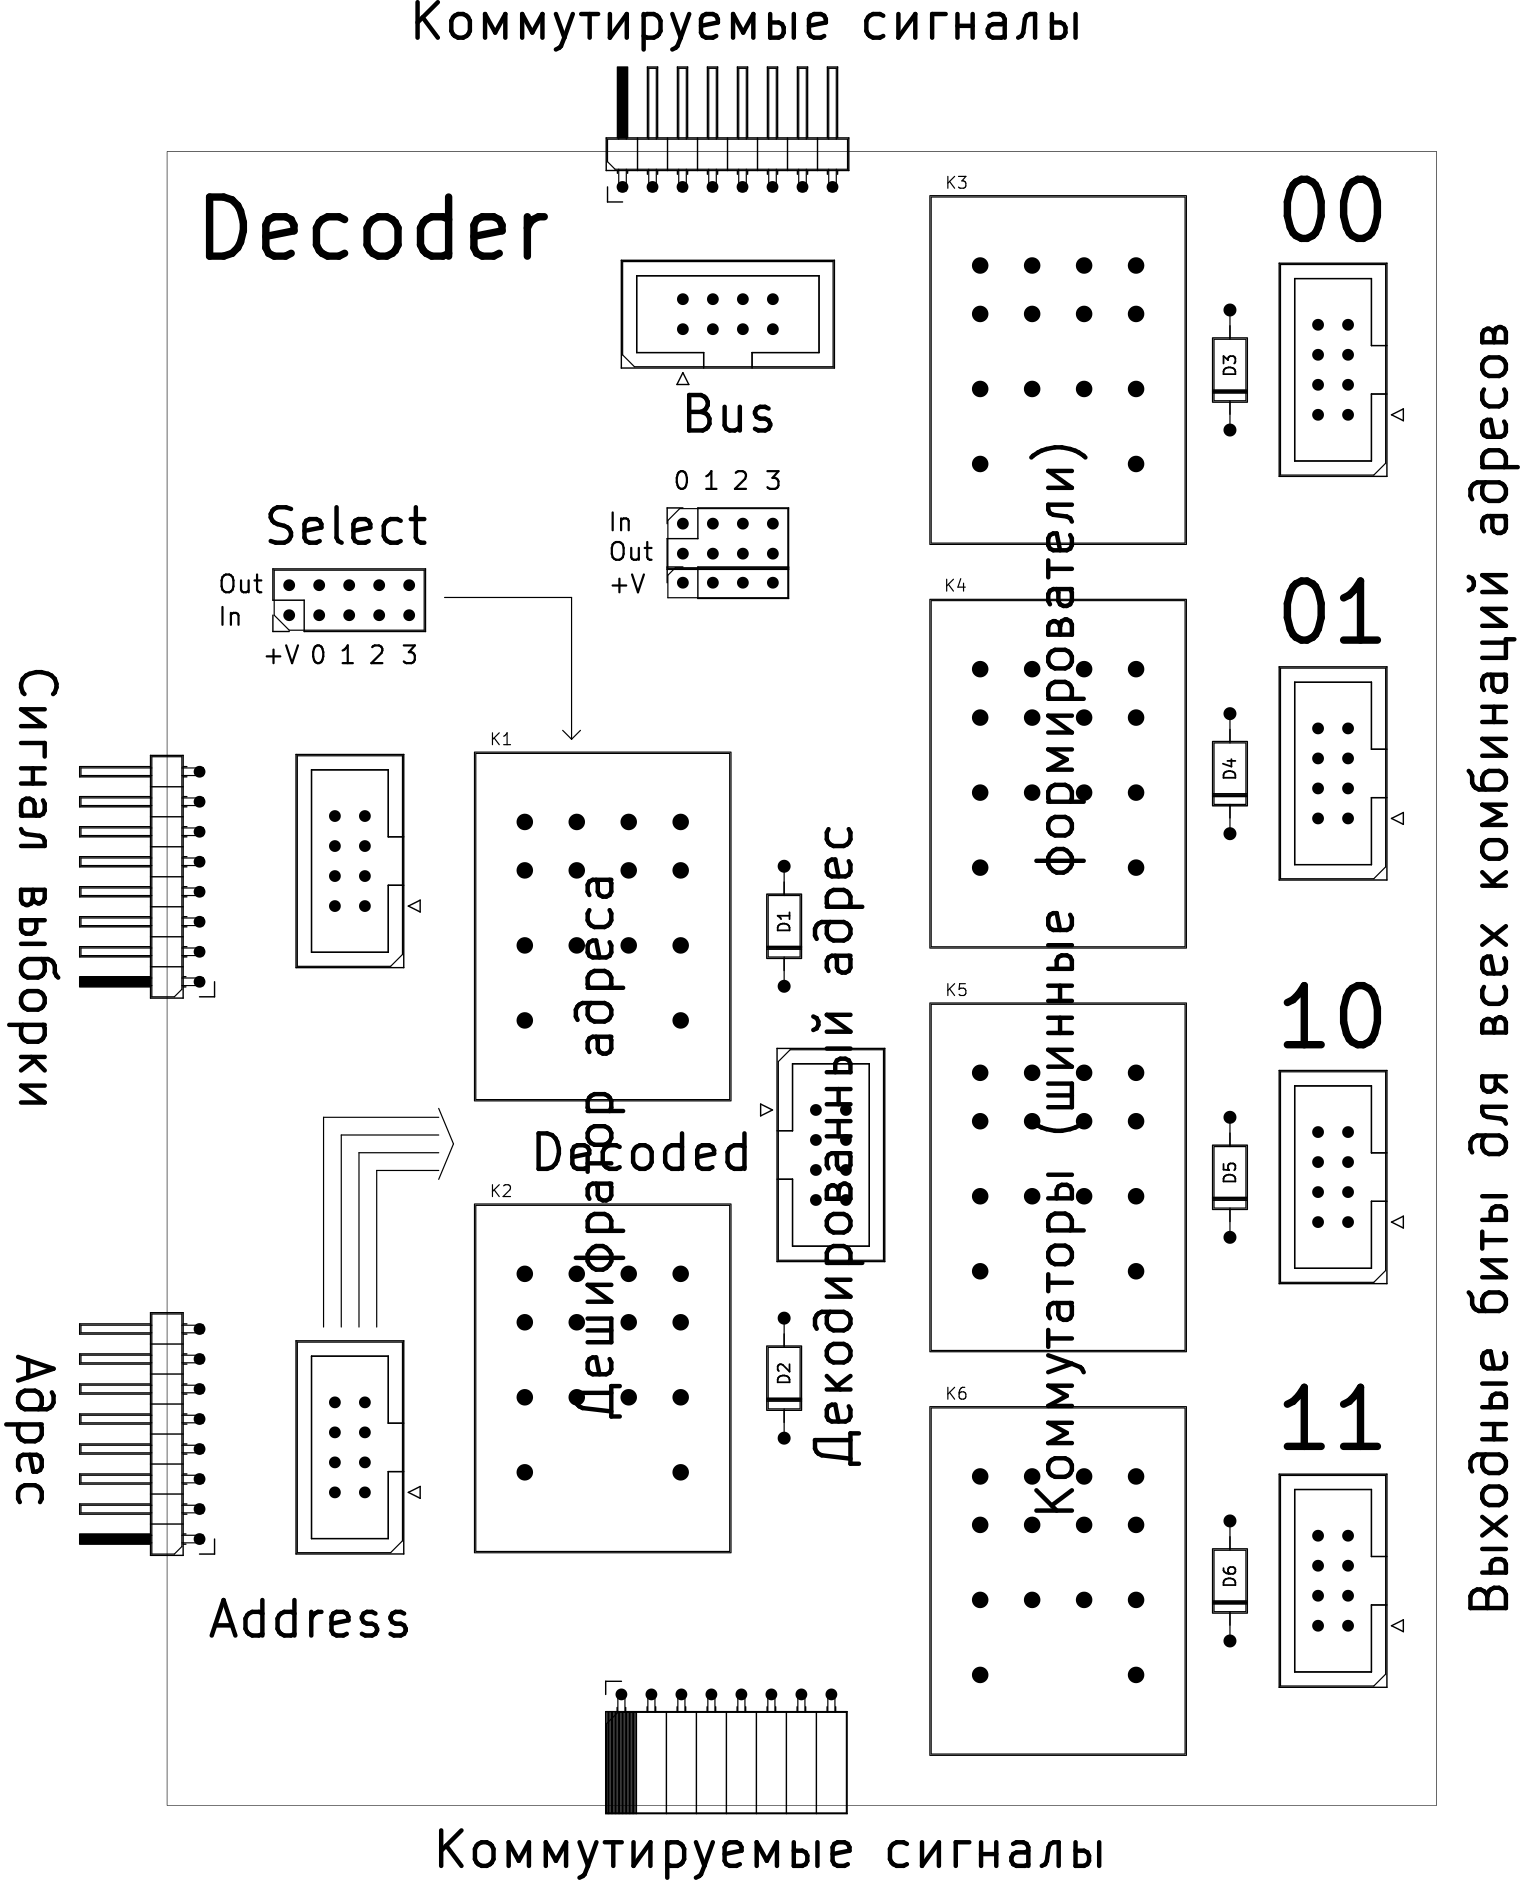
\includegraphics{../modules-png/decoder-pcb.png}
\end{center}

\section{Практикум}

\subsection{Устройство, угадывающее животных}

% a острые зубы
% b млекопитающее

% 0  пингвин
% 1  змея         a
% 2  жираф          b
% 3  леопард      a b

\subsection{Ещё больше животных}

Пять дешифраторов для каскадирования

% % WoS: 09-software.pdf page 20

% %            Животные: леопард, тигр, жираф, зебра, пингвин, альбатрос
% %Вопросы:
% %- острые зубы            x       x
% %- млекопитающее          x       x     x      x
% %- полосатое                      x            x
% %- летает                                                        x

% Вопросы:
% a острые зубы
% b млекопитающее
% c полосатое
% d летает


% Ответы:
% 0  пингвин
% 1  змея         a
% 2  жираф          b
% 3  леопард      a b
% 4                   c
% 6  зебра          b c
% 7  тигр         a b c
% 8  альбатрос          d
% 9               a     d
% 10                b   d
% 11 летучая мышь a b   d
% 12 оса              c d
% 13              a   c d
% 14                b c d
% 15              a b c d

\subsection{Выбор одного из четырёх значений с помощью дешифратора}

\subsection{Задачи}

\begin{itemize}
    \item Найдите животных, которыми можно было бы заполнить недостающие строки в таблице.
\end{itemize}
